\documentclass{standalone}
\usepackage{tikz}
\usetikzlibrary{backgrounds}
\usepackage{xcolor}
\definecolor{plotblue}{RGB}{100, 100, 255}
%\definecolor{myblue}{RGB}{8,164,214}
\definecolor{myred}{RGB}{143,42,41}
\definecolor{forestgreen}{RGB}{34,139,34}
\definecolor{highdive}{RGB}{10,169,194}

\begin{document}
	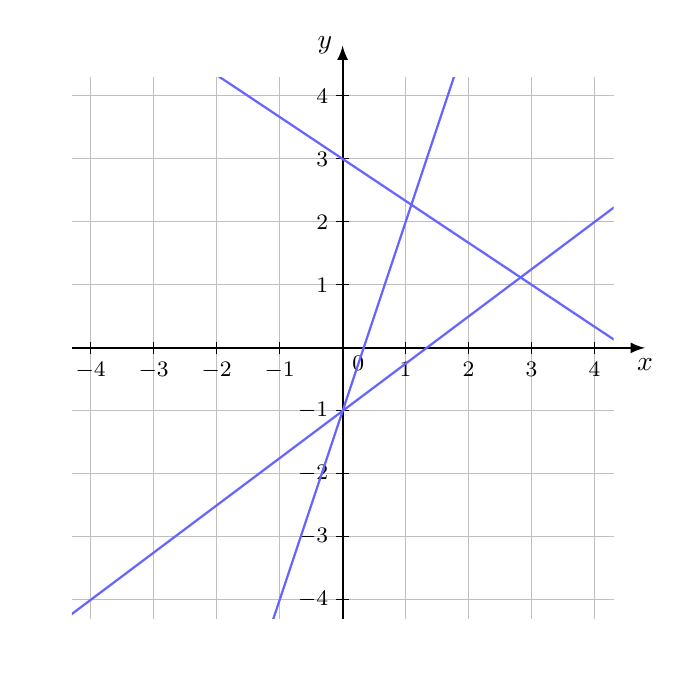
\begin{tikzpicture}[cross/.style={draw, cross out, minimum size=2*(#1-1pt), inner sep=0pt, outer sep=0pt}, x=10mm, y=10mm,
		>=latex,   %Voreinstellung für Pfeilspitzen
		font= \footnotesize, scale=0.8]
		\begin{scope}[on background layer]
			\fill[white] (-5,-5) rectangle (5,5);
		\end{scope}
		%Raster zeichnen
		\draw [color=gray!50]  [step=10mm] (-4.3,-4.3) grid (4.3,4.3);
		% Achsen zeichnen
		\draw[->,thick] (-4.3,0) -- (4.8,0) node[right, below] {\normalsize $x$};
		\draw[->,thick] (0,-4.3) -- (0,4.8) node[above, left] {\normalsize $y$};
		% Achsen beschriften
		\foreach \x in {-4,...,-2,-1,1,2,...,4} \draw (\x,-.1) -- (\x,.1) node[below=4pt] {$\x$};
		\foreach \y in {-4,...,-2,-1,1,2,...,4} \draw (-.1,\y) -- (.1,\y) node[left=4pt] {$\y$};
		% Besserer Ursprung
		\draw[color=black] (0pt,-7pt) node[right] {$0$};
		%Funktionen zeichnen:
		\clip(-4.3,-4.3) rectangle (4.3,4.3); %Bildbereich
		\draw[plotblue,thick,samples=200] plot (\x, {-0.666*(\x)+3});
		\draw[plotblue,thick,samples=200] plot (\x, {0.75*(\x)-1});
		\draw[plotblue,thick,samples=200] plot (\x, {3*(\x)-1});
		%Beschriftung
		%\node[myred]  at (3.1,-2.3) {$f:y=x^5-6x^3+1.8x$};
	\end{tikzpicture}


\end{document}